\subsection{Fonctionnalité 7}
La fonctionnalité 7 permettra d'envoyer un e-mail de rappel à l'établissement et au contact dans l'établissement (si son adresse électronique est différente de celle de l'établissement), une semaine avant l'intervention. Le texte de ce message sera à définir avec \nomClient{} et à faire valider par le responsable des plaideurs. \\

% Figure : version 1.00, date 24/02/16, auteur Michel Cressant
\begin{figure}[H]
	\centering
	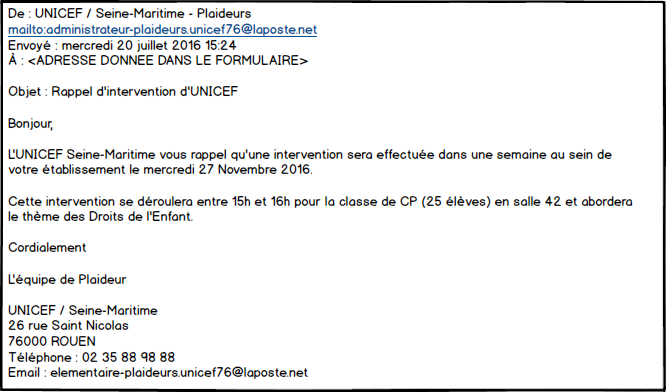
\includegraphics[scale=0.675]{images/maquettes/fonctionnalite7MailDeRappelPourLEtablissement.png}
	\caption{Maquette~: Email de rappel d'intervention pour un établissement}
\end{figure}

Trois jours avant l'intervention, le plaideur recevra un e-mail de rappel avec les informations associées (date, heure, lieu, thème, nombre d'élèves, remarques, niveau des élèves). 
\\

% Figure : version 1.00, date 24/02/16, auteur Michel Cressant
\begin{figure}[H]
	\centering
	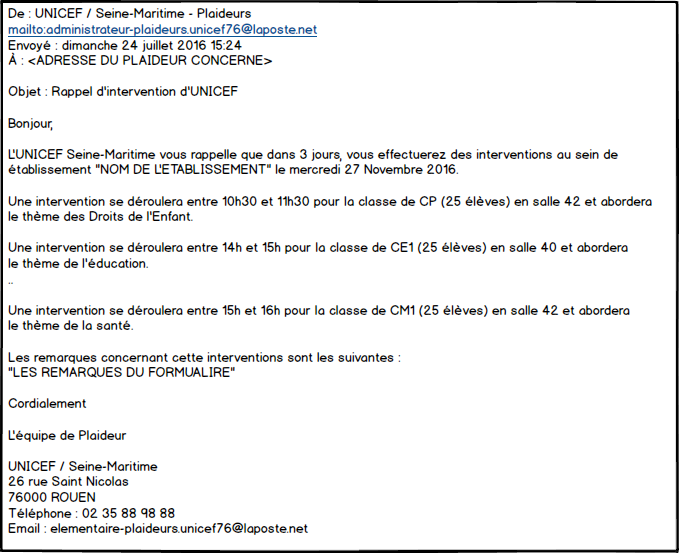
\includegraphics[scale=0.65]{images/maquettes/fonctionnalite7MailDeRappelPourLePlaideur.png}
	\caption{Maquette~: Email de rappel d'intervention pour le plaideur}
\end{figure}

\begin{figure}[H]
	\centering
	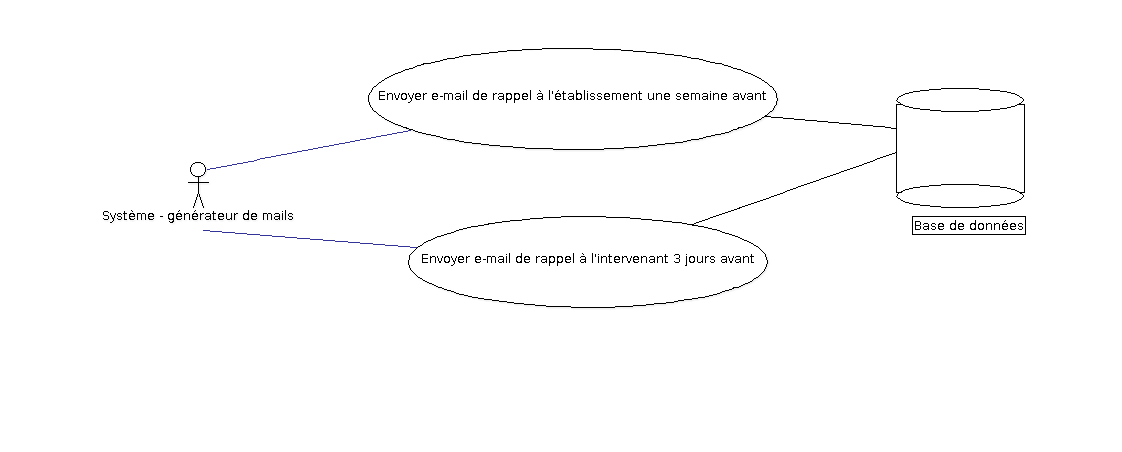
\includegraphics[scale=0.4]{images/casDUtilisation/fonctionnalite7Rappels.png}
	 \caption{Cas d'utilisation~: Envoyer des emails de rappels}
	 \label{envoiRappel}
\end{figure}